%!TEX root = ../rapport.tex
%!TEX encoding = UTF-8 Unicode
% Chapitres "Annexes"

% modifié par Francis Valois, Université Laval
% 31/01/2011 - version 1.0 - Création du document
\chapter{Annexes}
\label{s:annexes}

\section{Diagramme des cas d'utilisation}

\begin{figure}[htp]
  \caption{Diagramme des cas d'utilisation}
  \centering
  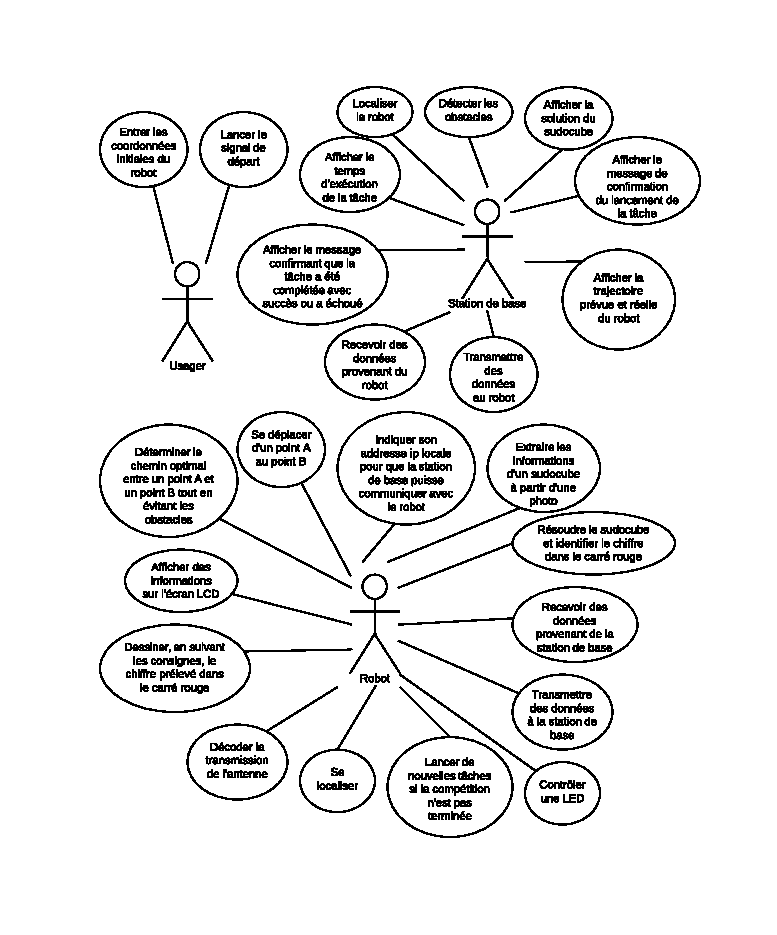
\includegraphics[scale=1, trim = 50 50 50 0]{fig/use_cases_diagram.pdf}
  \label{use_cases_diagram}
\end{figure}

\section{Code test pour affichage sur LCD} \label{s:code_LCD}
\subsection{ecran.h}
\begin{lstlisting}[language=C]
#ifndef ECRAN_H_
#define ECRAN_H_

#include "inc/hw_ints.h"
#include "inc/hw_memmap.h"
#include "inc/hw_types.h"
#include "driverlib/debug.h"
#include "driverlib/gpio.h"
#include "driverlib/interrupt.h"
#include "driverlib/rom.h"
#include "driverlib/timer.h"
#include "inc/lm3s9b92.h"

//definition de trucs qu vont etre pratiques

//#define STCTRL (*((volatile unsigned long *)0xE000E010))
//#define STRELOAD (*((volatile unisgned long *)0xE000E014))
//#define attend(t) SysCtlDelay((SysCtlClock()/3)/(1000/t))


#define ECRAN_DATA GPIO_PORTE_DATA_R
#define ECRAN_CTRL GPIO_PORTA_DATA_R
//volatile unsigned long ulLoop;
	
//bit de data du LCD
#define ECRAN_D0 0x01 //PE0
#define ECRAN_D1 0x02 //PE1
#define ECRAN_D2 0x04 //PE2
#define ECRAN_D3 0x08 //PE3 
#define ECRAN_D4 0x10 //PE4
#define ECRAN_D5 0x20 //PE5
#define ECRAN_D6 0x40 //PE6
#define ECRAN_D7 0x80 //PE7

//bit de control du LCD
#define ECRAN_RS 0x01 //PA0  reset
#define ECRAN_RW 0x02 //PA1  read/write
#define ECRAN_EN 0x04 //PA2  enable
#define ECRAN_BF 0x08 //PA3 "busy flag", indique que l'ecran est occupe

//volatile unsigned long ulLoop;
void ecranClear(void);
void ecranInit(void);
void ecranWriteChar(char caractere);
void ecranWriteLine(char * line, unsigned short size);
void ecranSetPosCursor(short pos);
void ecranAttend(void);
void ecranControl(unsigned long input);

#endif /*ECRAN_H_*/

\end{lstlisting}

\subsection{ecran.c}
\begin{lstlisting}[language=C]
#include "ecran.h"


/*
* Cette fonction permet de s'assurer que l'ecran n'est pas occupe avant d'ecrire 
 */
void ecranAttend(void)
{
    ECRAN_CTRL &= ~(ECRAN_RS); // RS = 0
    ECRAN_CTRL |= ECRAN_RW; // RW = 1
    volatile unsigned long busyflag = ECRAN_CTRL & ECRAN_BF;
    while (busyflag != 0) //on regarde le busyflag pour s'assurer que l'ecran est pas occupe
    { 
            busyflag = GPIO_PORTD_DATA_R & ECRAN_BF;
    }
     return;
}

/*
 * Cette fonction execute la routine d'initialisation de l'ecran dans le mode qu'on veut
 */
void ecranInit(void)
{
    ecranControl(ECRAN_D5 | ECRAN_D4 | ECRAN_D3 | ECRAN_D2);
    ecranControl(ECRAN_D3 | ECRAN_D2 | ECRAN_D1);
}

/*
 * Cette fonction permet de faire des commandes tel que l'initalisation, changement de positions et 
 * trucs du genre, tout ce qui est pas l'ecriture de caracteres sur l'ecran
 */
void ecranControl(unsigned long input)
{
ecranAttend();
 volatile unsigned long ulLoop;
ECRAN_DATA = input; //on met notre entree sur le port de donnees
ECRAN_CTRL &=~(ECRAN_RS | ECRAN_RW); //reset et read/write a zero pour pas qu'il re-ecrive par erreur
ECRAN_CTRL ^= ECRAN_EN;
ulLoop = SYSCTL_RCGC2_R;
        for (ulLoop = 0; ulLoop < 200; ulLoop++) 
        {
             // on met un delai pour que le LCD puisse voir le enable
        }
ECRAN_CTRL ^=ECRAN_EN;
ulLoop = SYSCTL_RCGC2_R; 
        for (ulLoop = 0; ulLoop < 200; ulLoop++) 
        {
        // on attend un peu pour que l'instruction s'execute avant de changer la pin 7
        }
 
ECRAN_DATA &= ~(ECRAN_D7); //on reset la pin 7 parce elle output aussi le busy flag et ont pas veux etre pogner dans ecranAttend()
}



/*
 * Cette fonction efface le contenu de l'ecran
 */
void ecranClear(void)
{
    ecranControl(ECRAN_D0);
    volatile unsigned long ulLoop;
    
    for (ulLoop = 0; ulLoop < 2000; ulLoop++) 
    {
        //loop pour etre sur que ton est bien clearer
    }
}

/*
 * Cette fonction change la position du curseur d'ecriture de l'ecran
 */
void ecranSetPosCursor(short pos)
{
    ecranControl(GPIO_PIN_7 | pos);
}

/*
 * Cette fonction permet d'ecrire un caractere sur l'ecran
 */
void ecranWriteChar(char caractere)
{
    volatile unsigned long ulLoop;
    ecranAttend();
    ECRAN_DATA = caractere;
    ECRAN_CTRL &= ~(ECRAN_RW); //RW = 0
    ECRAN_CTRL |=  ECRAN_RS; // rs = 1
    ECRAN_CTRL ^=  ECRAN_EN; //En = 1
    ulLoop = SYSCTL_RCGC2_R;
    for (ulLoop = 0; ulLoop < 200; ulLoop++) 
    {
        //petit delai, juste pour etre sur
    }
    ECRAN_CTRL ^= ECRAN_EN; //En = 0
}


/*
 * Cette fonction permet d'ecrire une chaine de caracteres sur l'ecran
 */
void ecranWriteLine(char * line, unsigned short size) //todo
{
    unsigned short i=0;
    for(i=0; i <size;i++)
    {
         ecranWriteChar(line[i]);
    }
}

\end{lstlisting}

